\documentclass[a4paper,11pt]{article}


%%% fontenc
%\usepackage{fontspec,xunicode,xltxtra}
%\setmainfont{Times New Roman}
%\setsansfont{Source Sans Pro}
%\setmonofont{Source Sans Pro}

%%% xeCJK
\usepackage{xeCJK}
\setCJKmainfont[BoldFont=Adobe Heiti Std]{Adobe Song Std}
\setCJKsansfont[BoldFont=Adobe Heiti Std]{Adobe Song Std}
\setCJKmonofont[BoldFont=Adobe Heiti Std]{Adobe Song Std}
\XeTeXlinebreaklocale "zh"
\XeTeXlinebreakskip=0pt plus 1pt minus 0.1pt

\usepackage{xcolor}
\usepackage{graphicx}

%%% get total page number
\usepackage{lastpage}

%%% customized definition
\makeatletter
\def\sybtitle#1{\def\@sybtitle{#1}}
\def\sybauthor#1{\def\@sybauthor{#1}}
\def\sybdate#1{\def\@sybdate{#1}}
\sybtitle{}
\sybauthor{}
\sybdate{}
\def\sybmaketitle{
  \begin{center}
  \vspace*{.8in}
  {\huge\bfseries\@sybtitle}
  \par
  \vspace{.8in}
  {\Large\@sybauthor}
  \par
  \vspace{.2in}
  \@sybdate
  \vspace{.5in}
  \end{center}
}
\makeatother
\setlength{\parindent}{0pt}
\renewcommand{\today}{\number\month 月 \number\day 日, ~\number\year 年}
\def\lt{\textless}
\def\gt{\textgreater}
\renewcommand\contentsname{\bfseries 目~~录}
\newcommand\bs{\texttt{\symbol{'134}}} % input backslash sign
%\newcommand\bs{\string\} % same as above definition
\long\def\cmd#1{\par\vspace{.5em}\hspace*{2em}#1\vspace{.5em}\par}
\def\cstr#1{\texttt{\string#1}} % e.g. \cstr{\latex}
\long\def\runcode#1{\par\bigskip#1\bigskip\par}
% 我不想看到那么多的underful hbox,尤其是minted环境加上背景色之后
\hbadness=10000
% 适当放宽overful hbox的限制,运行2pt的溢出
\hfuzz=2pt
\parskip=3\lineskip


%%% change background color & add frame for enumerate enviroment
\usepackage{mdframed}
\newmdenv[backgroundcolor=blue!10,linewidth=0pt]{coloredframe}
\newenvironment{coloredenumerate}{
  \begin{coloredframe}
  \begin{enumerate}
}{
  \end{enumerate}
  \end{coloredframe}
}

%%% geometry
\usepackage[includehead,includefoot,hmargin=21mm,vmargin=10.5mm,
            headsep=12pt,headheight=25pt]{geometry}
%\usepackage[includehead,includefoot,hmargin=1.2in,vmargin=1in]{geometry}

%%% fancyhdr
\usepackage{fancyhdr}
\makeatletter
\fancypagestyle{main} {
  \fancyhf{} % clear header & footer
  \fancyhead[L]{\bfseries\@sybtitle}
  \fancyhead[R]{\thepage/\pageref*{LastPage}}
  \renewcommand{\headrulewidth}{0.4pt} % header line
  \renewcommand{\footrulewidth}{0pt} % footer line
}
\fancypagestyle{header} {
  \fancyhf{} % clear header & footer
  \fancyfoot[C]{\roman{page}}
  \renewcommand{\headrulewidth}{0pt} % header line
  \renewcommand{\footrulewidth}{0pt} % footer line
}
\makeatother

\usepackage{titlesec}
\titleformat{\part}{\centering\Large\bfseries}{第\,\thepart\,部分}{1em}{}
\titleformat{\section}{\large\bfseries}{\thesection}{1em}{}
\titleformat{\subsection}{\normalsize\bfseries}{\thesubsection}{1em}{}
%\titlespacing*{章节命令}{左边距}{上文距}{下文距}[右边距]
\titlespacing*{\section}{0pt}{2\baselineskip}{\parsep}


\usepackage{hyperref}

%%% perfect source code display
\usepackage{minted}
%\usemintedstyle{colorful}
\definecolor{srcbg}{rgb}{0.95,0.95,0.95}
\newminted{java}{linenos,tabsize=4,bgcolor=srcbg}
\newminted{xml}{linenos,tabsize=4,bgcolor=srcbg}
\newminted{cpp}{linenos,tabsize=4,bgcolor=srcbg}
\newminted{bash}{linenos,tabsize=4,bgcolor=srcbg}
\newminted{latex}{linenos,tabsize=4,bgcolor=srcbg}
\newminted{scheme}{linenos,tabsize=4,bgcolor=srcbg}

\usepackage{amsmath}


\input{../styles/tikz_preamble}

\sybtitle{Algorithm Notes}
\sybauthor{孙延宾}
\sybdate{\today}

\begin{document}
  \tt % I love Typewriter font.
%%%%%%%% the title page and toc %%%%%%%%%%
  \pagestyle{header}
  \sybmaketitle
  \tableofcontents
  \newpage

%%%%%%% the main content %%%%%%%%%
  \pagestyle{main}
  \setcounter{page}{1}

  \section[rsync核心算法]{rsync核心算法}
  aaa

  \section[伙伴算法简易实现]{伙伴算法简易实现}
  \begin{center}
    % Requires \usepackage{graphicx}
    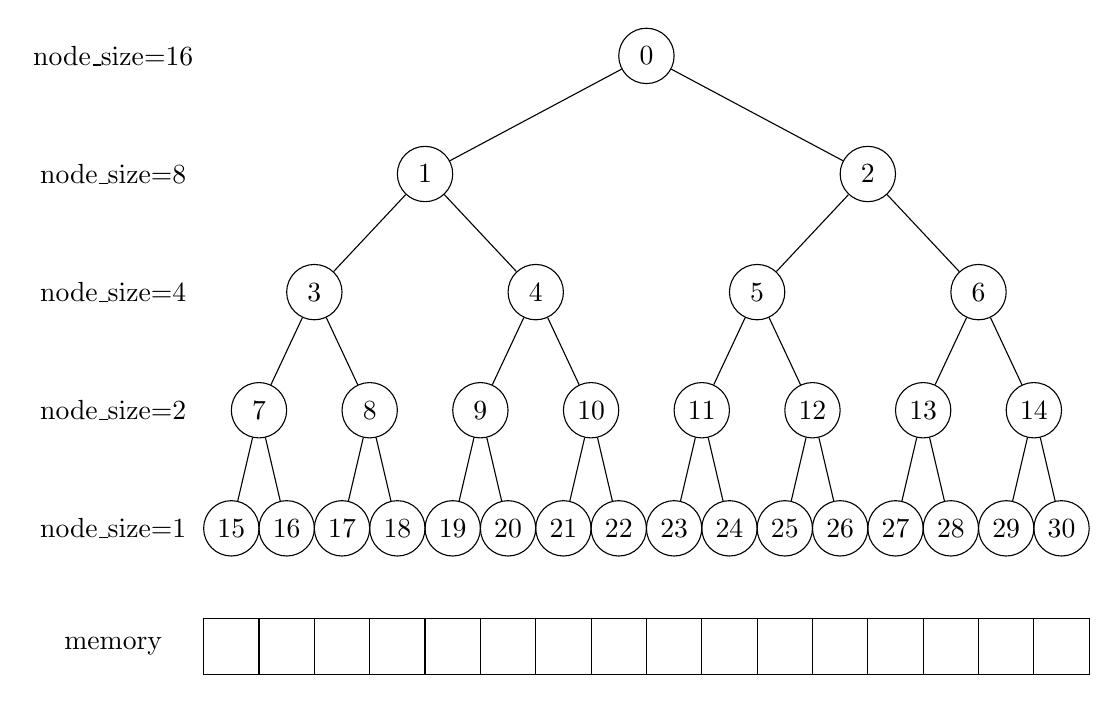
\begin{tikzpicture}
  [every node/.style={minimum size=20pt, inner sep=2pt},
   tree-node/.style={draw,circle},
   side-node/.style={},
   memo-node/.style={draw,rectangle},
   level 1/.style={sibling distance=160pt}, % 8 * 20pt
   level 2/.style={sibling distance=80pt}, % 4 * 20pt
   level 3/.style={sibling distance=40pt}, % 2 * 20pt
   level 4/.style={sibling distance=20pt}] % 1 * 20pt
  \node [tree-node] (root) {0}
    child {
      node [tree-node] {1}
        child {
          node [tree-node] {3}
            child {
              node [tree-node] {7}
                child {
                  node [tree-node] {15}
                    child [grow=down] {
                      node [memo-node] {} edge from parent[draw=none]
                        child [grow=left] {node [side-node] {memory} edge from parent[draw=none]}
                    }
                    child [grow=left] {
                      node [side-node] {node\_size=1} edge from parent[draw=none]
                        child [grow=up] {
                          node [side-node] {node\_size=2} edge from parent[draw=none]
                            child [grow=up] {
                              node [side-node] {node\_size=4} edge from parent[draw=none]
                                child [grow=up] {
                                  node [side-node] {node\_size=8} edge from parent[draw=none]
                                    child [grow=up] {
                                      node [side-node] {node\_size=16} edge from parent[draw=none]
                                    }
                                }
                            }
                        }
                    }
                }
                child {
                  node [tree-node] {16}
                    child [grow=down] {node [memo-node] {} edge from parent[draw=none]}
                }
            }
            child {
              node [tree-node] {8}
                child {
                  node [tree-node] {17}
                    child [grow=down] {node [memo-node] {} edge from parent[draw=none]}
                }
                child {
                  node [tree-node] {18}
                    child [grow=down] {node [memo-node] {} edge from parent[draw=none]}
                }
            }
        }
        child {
          node [tree-node] {4}
            child {
              node [tree-node] {9}
                child {
                  node [tree-node] {19}
                    child [grow=down] {node [memo-node] {} edge from parent[draw=none]}
                }
                child {
                  node [tree-node] {20}
                    child [grow=down] {node [memo-node] {} edge from parent[draw=none]}
                }
            }
            child {
              node [tree-node] {10}
                child {
                  node [tree-node] {21}
                    child [grow=down] {node [memo-node] {} edge from parent[draw=none]}
                }
                child {
                  node [tree-node] {22}
                    child [grow=down] {node [memo-node] {} edge from parent[draw=none]}
                }
            }
        }
    }
    child {
      node [tree-node] {2}
        child {
          node [tree-node] {5}
            child {
              node [tree-node] {11}
                child {
                  node [tree-node] {23}
                    child [grow=down] {node [memo-node] {} edge from parent[draw=none]}
                }
                child {
                  node [tree-node] {24}
                    child [grow=down] {node [memo-node] {} edge from parent[draw=none]}
                }
            }
            child {
              node [tree-node] {12}
                child {
                  node [tree-node] {25}
                    child [grow=down] {node [memo-node] {} edge from parent[draw=none]}
                }
                child {
                  node [tree-node] {26}
                    child [grow=down] {node [memo-node] {} edge from parent[draw=none]}
                }
            }
        }
        child {
          node [tree-node] {6}
            child {
              node [tree-node] {13}
                child {
                  node [tree-node] {27}
                    child [grow=down] {node [memo-node] {} edge from parent[draw=none]}
                }
                child {
                  node [tree-node] {28}
                    child [grow=down] {node [memo-node] {} edge from parent[draw=none]}
                }
            }
            child {
              node [tree-node] {14}
                child {
                  node [tree-node] {29}
                    child [grow=down] {node [memo-node] {} edge from parent[draw=none]}
                }
                child {
                  node [tree-node] {30}
                    child [grow=down] {node [memo-node] {} edge from parent[draw=none]}
                }
            }
        }
    };
\end{tikzpicture}
    %\caption{buddy system}\label{fig:buddy}
  \end{center}


  从伙伴算法看满二叉树的一些特性:
  \begin{description}
    \item[total\_leaf\_size] 满二叉树的叶子节点总数
    \item[level] 满二叉树的层级,范围0-max\_depth
    \item[node\_size] 每个level上节点的size
    \item[index] 某个节点在满二叉树数组中的索引
    \item[offset] 某一个节点对应的内存单元映射到叶子节点数组中的下标(offset)
  \end{description}
  total\_leaf\_size是已知的,即buddy system管理的内存单元总数。
  $$ max\_depth = \log_2total\_leaf\_size$$
  每个level上第一个左子树的index为$2^{level} - 1$
  \begin{align*}
    offset & = [index - (2^{level} - 1)] * node\_size \\
           & = (index + 1) * node\_size - 2^{level} * node\_size \\
           & = (index + 1) * node\_size - 2^{level} * 2^{max\_depth - level} \\
           & = (index + 1) * node\_size - 2^{max\_depth} \\
           & = (index + 1) * node\_size - total\_leaf\_size \\
  \end{align*}
  可见,无论哪个level,第一个左子树(最左边的节点)对应到叶子节点数组中的下标总是0.

  \section[字符串匹配的KMP算法]{字符串匹配的KMP算法}

  \section[字符串匹配的Boyer-Moore算法]{字符串匹配的Boyer-Moore算法}
  
  \section[寻找小于N的所有素数]{寻找小于N的所有素数}
  Sieve筛选算法用于寻找小于N的所有素数。\par
  \inputminted[linenos,tabsize=4,bgcolor=srcbg]{cpp}{srcdir/Sieve.c}
  
  筛选的方法是:\\
  首先去掉2的倍数,然后去掉3的倍数,然后去掉4的倍数,然后,...,
  直到去掉所有sqrt(n)的倍数,如下表:\par
  \begin{tikzpicture}
    \matrix [matrix of nodes]
    {
      2*\textcolor{red}{2} & 3*\textcolor{red}{2} & 4*\textcolor{red}{2} & 5*\textcolor{red}{2} & $\cdots$ & $\frac{n}{2}$ \\
      2*\textcolor{red}{3} & 3*\textcolor{red}{3} & 4*\textcolor{red}{3} & 5*\textcolor{red}{3} & $\cdots$ & $\frac{n}{3}$ \\
      2*\textcolor{red}{4} & 3*\textcolor{red}{4} & 4*\textcolor{red}{4} & 5*\textcolor{red}{4} & $\cdots$ & $\frac{n}{4}$ \\
      2*\textcolor{red}{5} & 3*\textcolor{red}{5} & 4*\textcolor{red}{5} & 5*\textcolor{red}{5} & $\cdots$ & $\frac{n}{5}$ \\
    };
  \end{tikzpicture}
  
  一般来说,任意一个小于sqrt(n)的数p,我们要去掉:\\
  2*p, 3*p, 4*p, 5*p, $\cdots$, p*p, (p+1)*p, (p+2)*p, $\cdots$\\
  观察一下可以发现,p*p以前的数字,在处理2、3、4、5、$\cdots$、(p-1)*p的倍数时
  都已经去掉了,所以对于p,我们从p*p开始移除。
  
  另外,为何只处理小于等于sqrt(n)的数字呢(上表中一直处理到n),从上面的说明可以知道,
  如果$p>sqrt(n)$,$p*p>n$,无需处理,而p*p之前的数字都已经移除了,
  也无需处理,所以如果$p>sqrt(n)$,则p无需处理。
  
  该方法的缺点是占用内存太大!

  \part[位操作算法实例]{位操作算法实例}
  aaa



\end{document}
